%Copyright 2011 Newcastle University
%
%   Licensed under the Apache License, Version 2.0 (the "License");
%   you may not use this file except in compliance with the License.
%   You may obtain a copy of the License at
%
%       http://www.apache.org/licenses/LICENSE-2.0
%
%   Unless required by applicable law or agreed to in writing, software
%   distributed under the License is distributed on an "AS IS" BASIS,
%   WITHOUT WARRANTIES OR CONDITIONS OF ANY KIND, either express or implied.
%   See the License for the specific language governing permissions and
%   limitations under the License.

\begin{chapter}{\label{cha:quickstart}Quick start guide}
  This chapter is intended as a quick start guide for those who are unfamiliar
  with \numbas.

  We shall describe the basics of constructing an exam and running it, without
  going into significant technical details.  By the end of this chapter you
  should have a simple, yet fully functioning, exam.

  \section{\label{sec:examfile}Creating the example exam}
  All aspects of an exam, including questions, variables, marks, answers, etc.,
  are described in a \codefile{.exam} file, which is a plain text file written
  in a simple markup language.

  In the \codefile{exam} directory you will find a file called
  \codefile{example.exam} (see listing~\ref{lst:example}), which describes a
  simple exam with one question containing two parts.  The example exam also
  includes an image in the question statement.  This image is stored in the
  resources directory for the exam.
  %
  \lstset{
    basicstyle=\ttfamily\footnotesize,
    numbers=left,
    numberstyle=\tiny,
    breaklines=true,
    breakatwhitespace=true
  }
  \lstinputlisting[caption={Example exam.}, label={lst:example}]{../../exams/example.exam}
  %
  We shall explain the various aspects of the markup in
  chapter~\ref{cha:examformat} and subsequent chapters, but for now, we can
  run this file through the exam interpreter to ``compile'' the exam,
  and produce a collection of HTML and JavaScript files.

  In a command prompt change to the directory where \numbas\ is unpacked, then
  run\footnote{On some systems it is possible for multiple versions of Python
  to co-exist.  If version 3.1 is not the default on your system, then you may
  need to use another command instead of \texttt{python}.  For example, on
  Debian and Ubuntu you might need to use \texttt{python3.1}, provided that the
  package \textit{python3} is installed.}

  %
  \begin{Verbatim}
    python bin/numbas.py exams/example.exam
  \end{Verbatim}
  %
  When the compilation finishes, you will see a message telling you that the
  exam has been created in \codefile{output/example}.

  Now, from a web browser, open the file \codefile{output/example/index.html}.
  You should then see a screen which looks like
  figure~\ref{fig:example_screen1}.
  %
  \begin{figure}[ht]
    \centering
    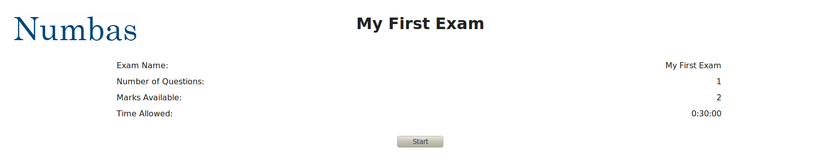
\includegraphics[scale=0.5]{fig/example_screen1}
    \caption{\label{fig:example_screen1}
      The first screen you see when opening the example exam.
    }
  \end{figure}
  %
  Information about the exam, \eg name, number of questions, available marks,
  time limits, etc., is shown on this page.
  
  Click the \codebutton{Start} button to begin the exam, and you will see the
  first question presented to you, as in figure~\ref{fig:example_screen2}.
  %
  \begin{figure}[ht]
    \centering
    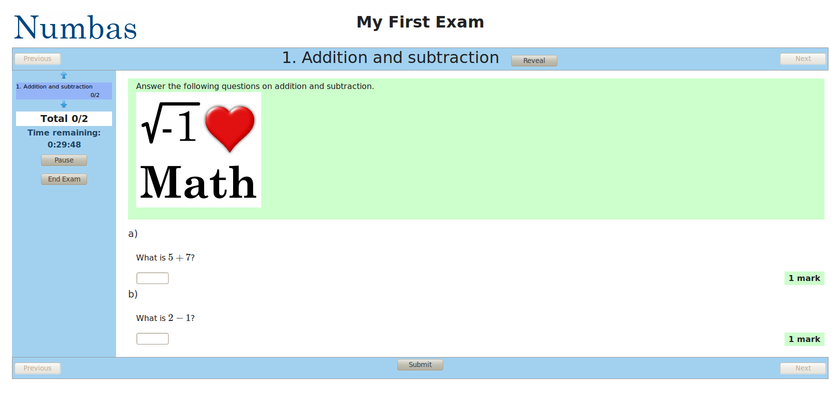
\includegraphics[scale=0.5]{fig/example_screen2}
    \caption{\label{fig:example_screen2}
      The first question of the exam.
    }
  \end{figure}
  %
  Each question of an exam is shown on a separate page, and navigation between
  questions is possible either by clicking the
  \codebutton{Previous}/\codebutton{Next} buttons, or by using the question
  list toward the left hand side of the page.  In the question list, the up and
  down arrow icons, or the mouse scroll wheel, can be used to scroll through
  questions if there are too many to show.

  The \codebutton{Reveal} button is used to show a ``worked solution'' to the
  current question, written by the question author.

  The question statement is shown in the green box at the beginning of the
  question, and question parts are shown underneath.

  Enter the answers in the boxes, and then press the \codebutton{Submit} button
  at the bottom of the page.  If your answers are correct, then you will see a
  green tick, and your score for this question, next to the \codebutton{Submit}
  button.  The question list will also be updated to show a tick, and your
  mark.  The total mark for the exam is also updated.

  If all of your answers are incorrect, then a red cross is shown; if some of
  your answers are correct, and some incorrect, a blue percent sign is shown,
  but you are not told which of your answers are incorrect.

  Now click the \codebutton{End Exam} button.  You are presented with a screen
  similar to figure~\ref{fig:example_screen3}.
  %
  \begin{figure}[ht]
    \centering
    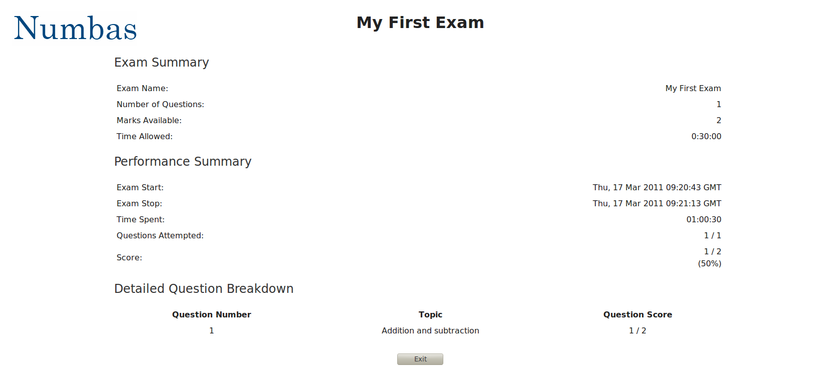
\includegraphics[scale=0.5]{fig/example_screen3}
    \caption{\label{fig:example_screen3}
      The performance summary page of the exam.
    }
  \end{figure}
  %
  This page shows the exam details again, and a breakdown of your performance
  in the exam.  Finally, clicking the \codebutton{Exit} button will finish the
  exam, and you can then close the browser window.

  \section{Creating your own exams}
  As you can see from the example, creating an exam is as simple as writing a
  plain text file, compiling it with the \codefile{numbas.py} interpreter,
  and opening the resulting files in a web browser.  A more complicated exam
  --- \codefile{mathssample.exam} --- demonstrating many aspects of the system,
  is also provided in the exams directory.

  Our recommendation would be to start off by using \codefile{example.exam},
  and modifying it to suit your needs.  Since questions are self-contained
  objects, they can be reused simply by copying and pasting from other exam
  files.

  \subsection{numbas.py}
  This file is the interpreter that translates the markup in a \codefile{.exam}
  file into a usable exam.  Running \verb"numbas.py -h" will show the
  help message, explaining the options available.
\end{chapter}
